\documentclass[lang=cn]{elegantpaper}

\title{Moore状态机}

\begin{document}

\maketitle



本题中输出需要完全由状态决定,因此需要设定不同的状态跳转方式。对于输出,只需在特定状态输出即可。为了输出的实时性,对输出采取 \lstinline{assign} 的方式进行赋值。

 \section{状态机运行模式}

转换图如 \figref{01} 。

\begin{figure}[htb]
    \centering
    \caption{转换图}\label{01}
    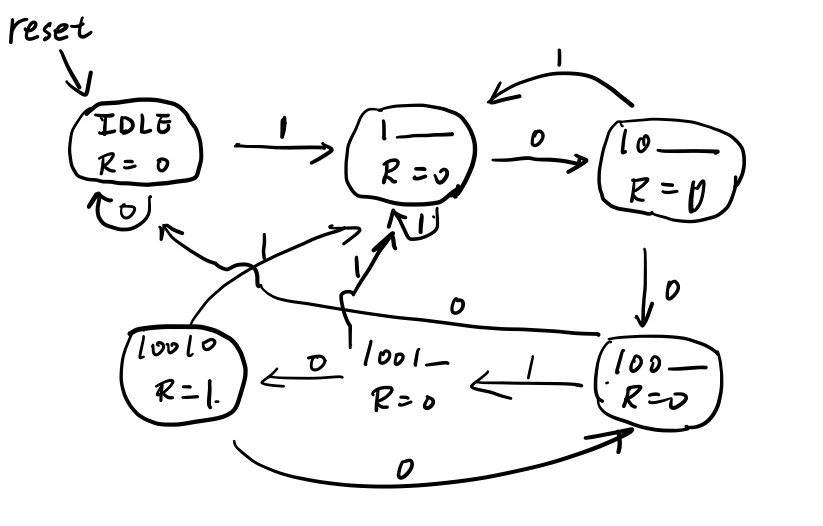
\includegraphics[width=0.6\textwidth]{trans.png}
\end{figure}




波形如 \figref{02} 。


\begin{figure}[htb]
    \centering
    \caption{波形图}\label{02}
    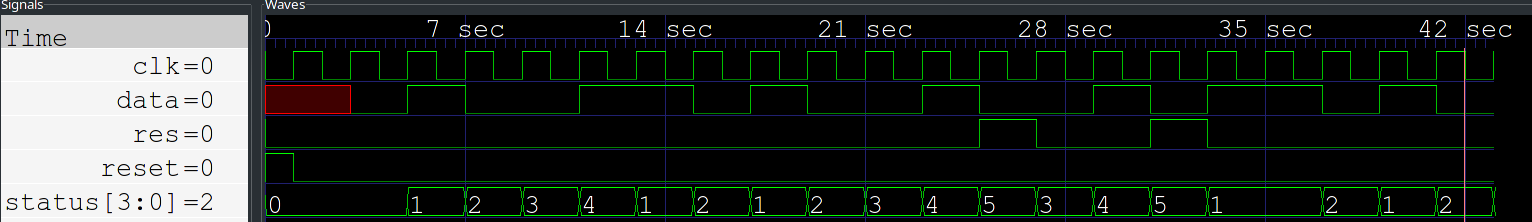
\includegraphics[width=0.6\textwidth]{wave.png}
\end{figure}


\end{document}